\section{Lecture 16: Conclusion of Module 3 }


\subsection{Introduction}
In this lecture we will look at simple replacement of continuous time RC circuit system with its equivalent discrete system. And also understand the purpose behind wanting to process signals digitally instead of in analog.
\subsection{Recap}
In the previous lecture we looked at an example of equivalent discrete time processing system for an RC circuit. The system we had looked at has the following feature
$\frac{1}{\tau}\equiv 3 kHz$ is the half power point and $\frac{1}{\tau}\equiv 9 kHz$ is the 10$\%$ power point.

\subsection{Construction of equivalent discrete system}
The DTFT of the discrete equivalent system H($\omega$) is essentially Fourier transform H($\Omega$) restricted to $-\Omega_m$ to $+\Omega_m$. We could take exact chopped(restricted) system of the RC response itself -$\pi$ to +$\pi$ treat that as frequency response of discrete system.


$$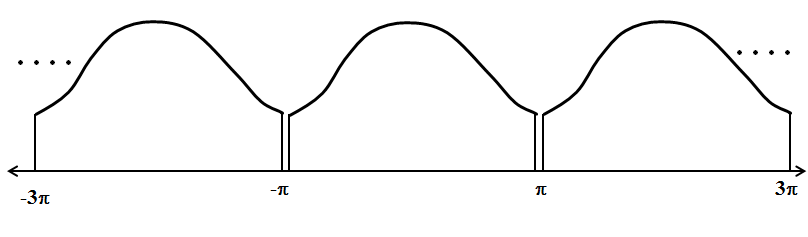
\includegraphics[width=0.5\textwidth]{H_w1_.png}$$
$$\mbox{Figure 1:DTFT of discrete equivalent system}$$




Or we could choose ideal low pass filter which behaves very similar to RC response.
$$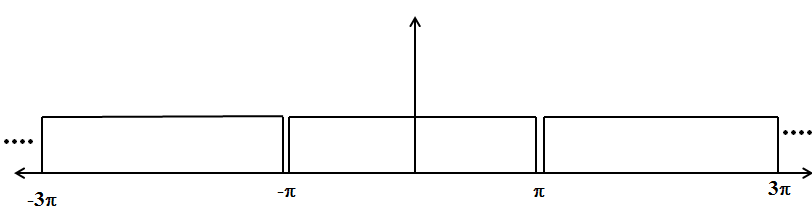
\includegraphics[width=0.7\textwidth,height=5cm]{H_w2_.png}$$
$$\mbox{Figure 2:Ideal low pass filter similar to H($\omega$)}$$
The second way is of course simpler. Low pass filter is characterised by cut off frequency. We can suitably choose the cut off at some frequency between 3 $kHz$ and 9 $kHz$ depending on where we are satisfied. We could choose 6 $kHz$ as cutoff for ideal low pass filter.

Ideal low pass filter with cut off $6 kHz$ is equivalent to discrete time system with the following frequency response.

$$\omega = \Omega T_s $$
Let us consider $T_s=\frac{1}{24 kHz}$
$$\omega = \frac{6}{24}2\pi = \frac{\pi}{2}$$
Ideal low pass filter on $\omega$ scale

$$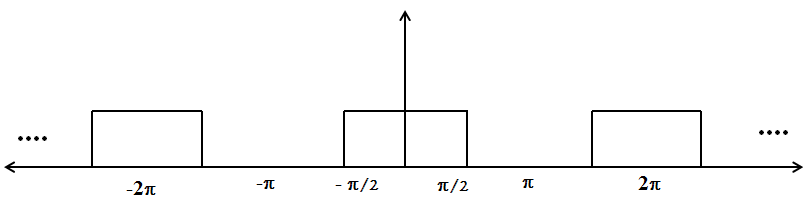
\includegraphics[width=0.9\textwidth]{H_w_.png}$$
$$\mbox{Figure 3:Ideal low pass filter with cut off 6 kHz on $\omega$ scale}$$

    $H(\omega)$ is DTFT of corresponding impulse response h[n].
    
    $$H(\omega)= \sum\limits_{n=-\infty}^{+\infty} h[n] e^{-j\omega n}$$
    
Note this is periodic with period 2$\pi$
$$H(\omega + 2\pi) = \sum\limits_{n=-\infty}^{+\infty} h[n]e^{-j(\omega+2\pi)n}$$
     $$H(\omega + 2\pi) = \sum\limits_{n=-\infty}^{+\infty} h[n]e^{-j\omega n}e^{-j2\pi n}$$
    Note $e^{-j2\pi n}$ =1 for all integer n and therefore the periodicity.
\subsection{Inverse Discrete Time Fourier Transform }


Think $H(\omega)$ as the Fourier transform of a continuous time impulse response sampled at unit frequency.

 Corresponding continuous time impulse response in the inverse Fourier transform  
 $$\frac{1}{2\pi} \int\limits_{-\pi}^{\pi} H(\omega)e^{j\omega t} \mbox{d$\omega$}$$.
 
We can get impulse response of the discrete system by replacing $t=n$.
Impulse response of DT system is given by inverse DTFT of $H(\omega)$,


$$h[n]=\frac{1}{2\pi}\int\limits_{-\pi}^{\pi} H(\omega) e^{j\omega n}\mbox{d$\omega$}$$

Exercise: 
Let $H(\omega) = 1$ for $-\frac{\pi}{2} \leq \omega \leq \frac{\pi}{2}$, else 0.

$$h[n] =\frac{1}{2\pi}\int\limits_{-\frac{\pi}{2}}^{\frac{\pi}{2}} 1.e^{j\omega n}\mbox{d$\omega$}$$
Evaluating seperately for $n=0$ and $n \neq 0$.
$$h[n]=\frac{1}{2\pi}\int\limits_{-\frac{\pi}{2}}^{\frac{\pi}{2}}1.\mbox{d$\omega$} , n=0 $$
$$=\frac{1}{2\pi}\int\limits_{-\frac{\pi}{2}}^{\frac{\pi}{2}}1.e^{j\omega n}\mbox{d$\omega$} , n\neq 0$$
After simple calculations we get the expression for h[n] as

$$h[n]=\frac{1}{2}, n=0$$
       $$=\frac{sin\frac{\pi}{2} n}{\pi n},n \neq 0$$
      

Keep in mind that we over simpilfied the RC circuit response. It is possible to find out the exact impulse response of the RC circuit chopped frequency response.

\subsection{Exact Impulse Response}

$$ H(\Omega)= \frac{1}{1+j\Omega \tau}$$
 $$\Omega =\frac{\omega}{T_s}$$

$$H(\omega) = \frac{1}{1+j\omega \frac{\tau}{T_s}} : -\pi \leq \omega \leq \pi$$
Recall we restricted the frequency response from $-\pi$ to $+\pi$
exact h[n] = Inverse DTFT of H($\omega$).


$$h[n]=\frac{1}{2\pi}\int\limits_{-\pi}^{\pi} \frac{e^{j\omega n}}{1+j\omega\frac{\tau}{T_s}} \mbox{d$\omega$}$$

Calculate h[n] and compare with low pass filter that we have taken.

\subsection{Conclusion of this module}

Continuous systems are found everywhere in real life.
Discrete systems occur sometimes and therefore continuous independent variable make lot of sense if you want to understand real life situation. In general it is continuous variable that dominates seemingly in the word around us.

We could of-course construct artificial discrete time system. Economic and financial are good examples.All systems that operate at certain points of the clock are good examples.

But continuous independent variable is much more difficult to understand and process. The convenience of processing discrete independent variable comes from the fact that all the discrete time operation can be done by storing the input samples in a computer, processing them on a computer with a discrete time system which is implemented in the form of a small program.
The moment you are in discrete time you can program it by having a loop that repeats at every instant n. A discrete time system can be implemented with modern computing devices. In a discrete system for an input sequence you can write a computer program to get the output sequence.
$$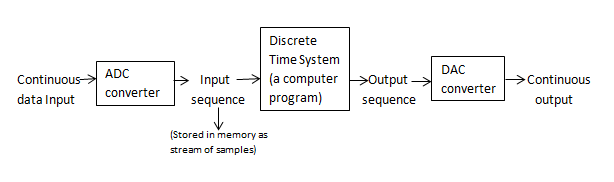
\includegraphics[width=1\textwidth]{adc.png}$$
Module 3 has given you the tools to interchange between discrete independent variable and continuous independent variable. By this time you must have noted that continuous independent time is reality and discrete independent time is convenience.

    



